%! Author = admin
%! Date = 2023/12/17

% Preamble
\documentclass[a4paper]{article}

% Packages
\usepackage[margin=1in]{geometry}
\usepackage[fontset=founder]{ctex}
\usepackage{anyfontsize}

\usepackage{graphicx,caption,subcaption}

\usepackage{amsmath,amssymb,mathabx}

\usepackage{algorithm,algorithmicx,algpseudocode,float}
\usepackage{lipsum}

\usepackage{multirow}

\usepackage{hyperref}

\graphicspath{{../figures/}}

\title{\textbf{数据结构实验报告}}
\author{姚苏航\qquad PB22061220}
\date{}

\newenvironment{breakablealgorithm}
{% \begin{breakablealgorithm}
    \begin{center}
        \refstepcounter{algorithm}% New algorithm
        \hrule height.8pt depth0pt \kern2pt% \@fs@pre for \@fs@ruled
        \renewcommand{\caption}[2][\relax]{% Make a new \caption
                {\raggedright\textbf{\ALG@name~\thealgorithm} ##2\par}%
            \ifx\relax##1\relax % #1 is \relax
            \addcontentsline{loa}{algorithm}{\protect\numberline{\thealgorithm}##2}%
            \else % #1 is not \relax
            \addcontentsline{loa}{algorithm}{\protect\numberline{\thealgorithm}##1}%
            \fi
            \kern2pt\hrule\kern2pt
        }
        }{% \end{breakablealgorithm}
        \kern2pt\hrule\relax% \@fs@post for \@fs@ruled
    \end{center}
}

% Document
\begin{document}
    \maketitle


    \section{问题描述}\label{sec:des}

    \subsection{实验题目}\label{subsec:q}
    {{利用哈希表统计两源程序的相似性。}}

    \subsection{基本要求}\label{subsec:req}
    {{对于两个C语言的源程序清单,
    用哈希表的方法分别统计两程序中使用C语言关键字的情况,
    并最终按定量的计算结果,得出两份源程序的相似性。}}

    \subsection{测试数据}\label{subsec:test}
    {{事先给出的file文件夹,包含关键词表和三份源程序文件,程序之间有相近的和差别大的。
    文件内容详见附录\ref{sec:appendix2}。}}


    \section{需求分析}\label{sec:need}

    \noindent{1.扫描给定的源程序,累计在每个源程序中 C 语言关键字出现的频度
        (为保证查找效率,建议自建哈希表的平均查找长度不大于2),
        通过这种方式扫描两个源程序,提取其特征向量。}

    \noindent{2.通过计算向量Xi和Xj的相似值来判断对应两个程序的相似性,
    相似值的判别函数计算公式为:}
    \begin{equation}
        S(X_i,X_j)=\frac{X_i^T\cdot X_j}{|X_i|\cdot|X_j|}\label{eq:equation}
    \end{equation}
    \noindent{\;\;\,\ 通过这种方式,可以初步判断两个源程序的相似性,如图\ref{fig:S}所示。
    其中 S 反映了两向量的夹角的余弦,当 S 趋近于 1 时,
    两向量夹角趋于 0 ,即两向量趋于相似,反之亦然。}
    \begin{figure}[htbp]
        \centering
        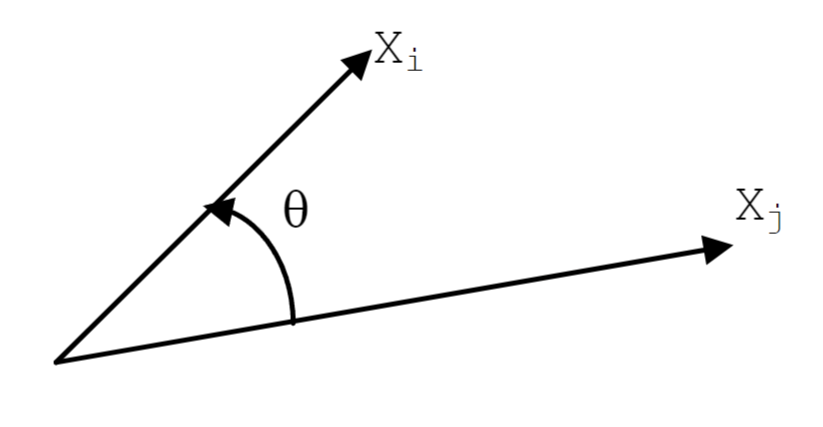
\includegraphics[height=120pt]{S}
        \caption{Similarity}\label{fig:S}
    \end{figure}

    \noindent{3.在有些情况下,S 不能很好地反映两向量的相似性,还需要进一步的考虑。
    例如,在 S 接近于 1 时,两向量的模的差距不能很好地被反映,如图\ref{fig:D}所示。
    因此引入几何距离 D ,用于反应两向量终点间的距离。}
    \begin{figure}[htbp]
        \centering
        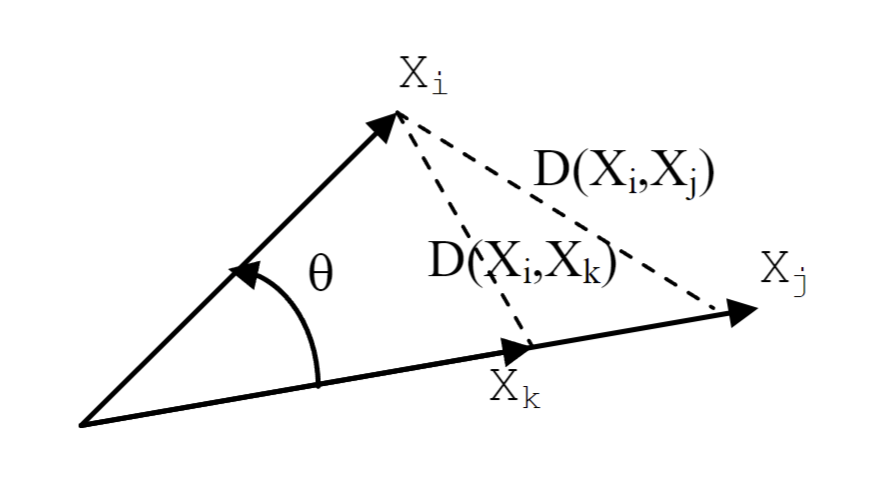
\includegraphics[height=120pt]{D}
        \caption{Distance}\label{fig:D}
    \end{figure}

    \noindent{4.通过分别比较很相近和差别很大的三个源代码,实践这种方法的有效性。}


    \section{概要设计}\label{sec:design1}

    \subsection{所用到得数据结构及其ADT}\label{subsec:adt}
    \begin{algorithm}
        %\textsl{}\setstretch{1.8}
        \renewcommand{\algorithmicrequire}{\textbf{Input:}}
        \renewcommand{\algorithmicensure}{\textbf{Output:}}
        \caption{STVMD based on STFT}
        \begin{algorithmic}[1]
            \Input $n \geq 0 \vee x \neq 0$
            \Output $y = x^n$
            \STATE $y \gets 1$
            \IF{$n < 0$}
            \STATE $X \gets 1 / x$
            \STATE $N \gets -n$
            \ELSE
            \STATE $X \gets x$
            \STATE $N \gets n$
            \ENDIF
            \WHILE{$N \neq 0$}
            \IF{$N$ is even}
            \STATE $X \gets X \times X$
            \STATE $N \gets N / 2$
            \ELSE[$N$ is odd]
            \STATE $y \gets y \times X$
            \STATE $N \gets N - 1$
            \ENDIF
            \ENDWHILE
        \end{algorithmic}\label{alg:algorithm}
    \end{algorithm}

    \subsection{主程序流程及其模块调用关系}\label{subsec:relate}

    \subsection{核心模块的算法伪码}\label{subsec:code}


    \section{详细设计}\label{sec:design2}

    \subsection{实现概要设计中的数据结构ADT}\label{subsec:adt2}

    \subsection{实现每个操作的伪码,重点语句加注释}\label{subsec:explain}

    \subsection{主程序和其他模块的伪码}\label{subsec:code2}


    \section{调试分析}\label{sec:debug}

    \subsection{问题分析与体会}\label{subsec:analysis}

    \subsection{时空复杂度分析}\label{subsec:analysis2}


    \section{使用说明}\label{sec:instrut}
    {{用户将事先准备好的关键词表(keyword.txt)和需要统计相似性的程序放入file文件夹中,
    运行时程序将通过关键词表建立哈希表,并通过查找哈希表构建两程序的向量,
    最后通过判别函数计算两程序相似性和向量的几何距离。}}

    {{在本项目中,使用事先给出的测试数据,
    准备三个编译和运行都无误的C程序,程序之间有相近的和差别大的,
    通过similar.c和different.c两个程序与main.c进行比较,
    可以直观展现出比较的效果。}}


    \section{测试结果}\label{sec:result}

    \subsection{输入数据}\label{subsec:in}
    {{输入数据从给出的测试文件中读取,
    读取keyword.txt文件生成哈希表,
    再分别读取main.c,similar.c,different.c并进行比较。}}

    \subsection{输出数据}\label{subsec:out}
    \noindent{输出结果显示在终端,内容如下:}

    \noindent{X\_(../file/similar.c):}

    \noindent{0 1 1 4 0 1 0 3 3 1 2 1 2 0 1 1 4}

    \noindent{X\_(../file/different.c):}

    \noindent{0 1 0 1 0 0 1 2 1 0 3 0 0 0 1 3 2}

    \noindent{X\_(../file/main.c):}

    \noindent{0 1 1 3 0 1 0 3 2 1 2 1 2 0 1 1 4}

    \noindent{ }

    \noindent{S\_(Sim\&Main):0.988174}

    \noindent{D\_(Sim\&Main):1.41421}

    \noindent{ }

    \noindent{S\_(Dif\&Main):0.740121}

    \noindent{D\_(Dif\&Main):4.89898}


    \appendix


    \section{实验源代码文件}\label{sec:appendix1}
    {{为方便查看,附录中的链接文件均为txt格式}}

    \href{../exp6/define.h.txt}{\underline{define.h}}

    \href{../exp6/main.cpp.txt}{\underline{main.cpp}}

    \href{../exp6/OpenHashing.h.txt}{\underline{OpenHashing.h}}

    \href{../exp6/OpenHashing.cpp.txt}{\underline{OpenHashing.cpp}}

    \href{../exp6/system.h.txt}{\underline{system.h}}

    \href{../exp6/system.cpp.txt}{\underline{system.cpp}}

    \href{../exp6/SimAsses.h.txt}{\underline{SimAsses.h}}

    \href{../exp6/SimAsses.cpp.txt}{\underline{SimAsses.cpp}}


    \section{实验用测试文件}\label{sec:appendix2}
    \href{../exp6/file/main.c.txt}{\underline{main.c}}

    \href{../exp6/file/different.c.txt}{\underline{different.c}}

    \href{../exp6/file/similar.c.txt}{\underline{similar.c}}

    \href{../exp6/file/keyword.txt}{\underline{keyword.txt}}


\end{document}
